\documentclass[tikz,border=10pt]{standalone}
\usepackage{tikz}
\usetikzlibrary{positioning,shapes.geometric,arrows.meta,calc,fit,backgrounds}
\usepackage{amsmath}

\begin{document}
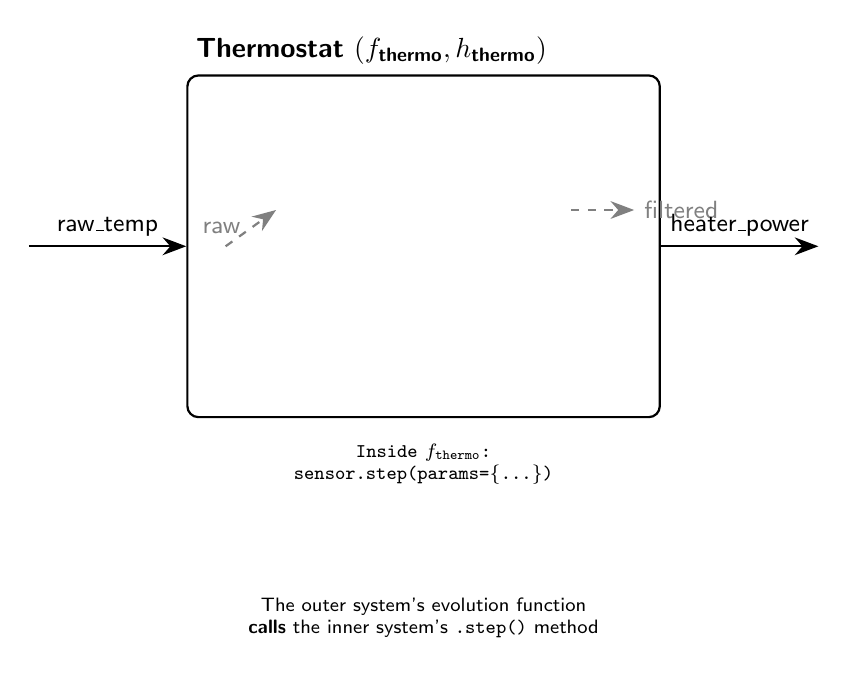
\begin{tikzpicture}[
    node distance=2cm,
    outer_block/.style={rectangle, draw, thick, fill=white, rounded corners, minimum height=4cm, minimum width=6cm, font=\sffamily\bfseries},
    inner_block/.style={rectangle, draw, fill=white, text width=3.5cm, text centered, rounded corners, minimum height=1.2cm, font=\sffamily},
    arrow/.style={-{Stealth[length=3mm]}, thick},
    signal/.style={font=\small\sffamily},
    label/.style={font=\small\sffamily\itshape}
]

% Inner system (Temperature Sensor)
\node[inner_block] (sensor) {Temperature Sensor\\[2pt]{\small $(f_{\text{sensor}}, h_{\text{sensor}})$}\\[2pt]{\scriptsize Exponential Filter}};

% Label showing it's wrapped
\node[above=0.3cm of sensor, label] (wrapped_label) {\textit{Inner DynamicalSystem}};

% State variables inside outer system
\node[below=0.8cm of sensor, font=\small\sffamily, text width=4cm, align=center] (state_vars) {
    State: \texttt{\{'filtered\_temp',}\\
    \texttt{'integral\_error'\}}
};

% Outer system boundary (Thermostat)
\node[outer_block, fit={(sensor) (wrapped_label) (state_vars)}] (thermostat) {};
\node[above right, font=\sffamily\bfseries] at (thermostat.north west) {Thermostat $(f_{\text{thermo}}, h_{\text{thermo}})$};

% Input and output coordinates
\coordinate[left=2cm of thermostat.west] (input);
\coordinate[right=2cm of thermostat.east] (output);

% Annotation showing .step() call
\node[below=0.2cm of thermostat.south, font=\scriptsize\ttfamily, text width=5.5cm, align=center] (annotation) {
    Inside $f_{\text{thermo}}$:\\
    \texttt{sensor.step(params=\{...\})}
};

% Input arrow
\draw[arrow] (input) -- node[above, signal] {raw\_temp} (thermostat.west);

% Internal data flow (showing wrapped call)
\coordinate (entry_point) at ($(thermostat.west) + (0.5, 0)$);
\draw[arrow, dashed, gray] (entry_point) -- node[left, signal, gray] {raw} (sensor.west);
\draw[arrow, dashed, gray] (sensor.east) -- ++(0.8, 0) node[right, signal, gray] {filtered};

% Output arrow
\draw[arrow] (thermostat.east) -- node[above, signal] {heater\_power} (output);

% Highlight box showing the wrapping concept
\node[below=1.2cm of annotation, font=\scriptsize\sffamily, text width=6cm, align=center] (concept) {
    The outer system's evolution function\\
    \textbf{calls} the inner system's \texttt{.step()} method
};

\end{tikzpicture}
\end{document}
